\documentclass[a4paper,12pt]{article}

%===================================================================================
% Paquetes
%-----------------------------------------------------------------------------------
\usepackage{amsmath}
\usepackage{float}
\usepackage{amsfonts}
\usepackage{amssymb}
\usepackage[utf8]{inputenc}
\usepackage{listings}
\usepackage[pdftex]{hyperref}
\usepackage{graphicx}

\usepackage{listings}
\usepackage{color}

\definecolor{dkgreen}{rgb}{0,0.6,0}
\definecolor{gray}{rgb}{0.5,0.5,0.5}
\definecolor{mauve}{rgb}{0.58,0,0.82}
\def\code#1{\texttt{#1}}

\lstset{frame=tb,
  language=Python,
  aboveskip=3mm,
  belowskip=3mm,
  showstringspaces=false,
  columns=flexible,
  basicstyle={\small\ttfamily},
  numbers=none,
  numberstyle=\tiny\color{gray},
  keywordstyle=\color{blue},
  commentstyle=\color{dkgreen},
  stringstyle=\color{mauve},
  breaklines=true,
  breakatwhitespace=true,
  tabsize=3
}

%-----------------------------------------------------------------------------------
% Configuración
%-----------------------------------------------------------------------------------
\hypersetup{colorlinks,%
	    citecolor=black,%
	    filecolor=black,%
	    linkcolor=black,%
	    urlcolor=blue}


\begin{document}

 

\title{ej6}

\begin{titlepage}
\centering
\vspace*{\fill}
\vspace*{0.5cm}
\huge\bfseries
Proyecto de Compilador de Cool\\
\vspace*{0.5cm}
\large Rodrigo García Gómez\\
Jorge Mederos Alvarado
\vspace*{\fill}
\end{titlepage}


\section*{Ejecución}
puede usar el siguiente comando en la consola, desde la carpeta $src$ para la ejecución del compilador.

\begin{lstlisting}
python -m coolpyler <archivo.cl>
\end{lstlisting}


\section*{Estructura}
Todo el código se encuentra dentro de la carpeta $coolplayer$, ubicada en $src$.

\begin{figure}[H]
\centering
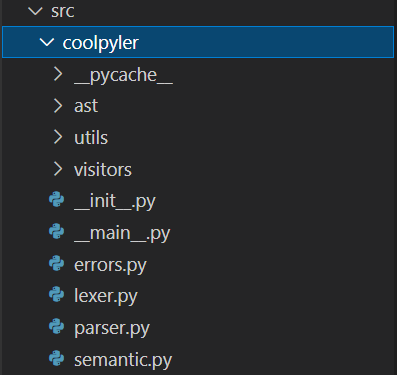
\includegraphics[width=0.9\linewidth]{./1}
\caption{}
\label{fig:1}
\end{figure}

El archivo $semantic.py$ es el que fue facilitado por los profesores en 3er año con código útil para la fase semántica tales como las clases \code{Type} y \code{Scope}, con modificaciones mínimas. Los archivos $lexer.py$ y $parser.py$ contienen, respectivamente, las clases necesarias para las fases de análisis lexicográfico y de parseo. Mientras que $errors.py$ contiene los tipos de errores que pueden ser recolectados por el compilador a través de sus diferentes fases, con texto acorde a cada situación. Las carpetas $ast$ y $visitors$ se muestran a continuación.

\begin{figure}[H]
\centering
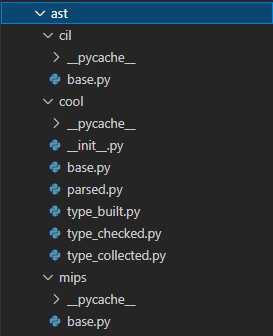
\includegraphics[width=0.9\linewidth]{./2}
\caption{}
\label{fig:2}
\end{figure}

En $ast$ se tienen los archivos con los árboles definidos para cada fase. En cada fase se tiene un ast base que tiene la forma básica a partir de la cual heredan los restantes. Para cil y mips sólo fue necesario un ast (base), pero en el caso de cool, fueron definidos varios ast´s de acuerdo a las necesiadades de entrada y salida de cada momento del chequeo semántico. Más adelante se explican a fondo los ast´s y su jerarquía.

\begin{figure}[H]
\centering
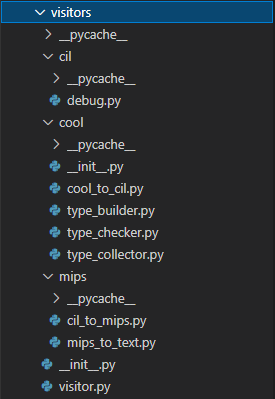
\includegraphics[width=0.9\linewidth]{./3}
\caption{}
\label{fig:3}
\end{figure}

En $visitors$ se encuentra la implementación de todas las fases del patrón visitor utilizado para recibir el código $cool$ parseado y generar código $mips$ a partir de él, pasando por la búsqueda de errores pertinente. En el caso de la carpeta $cil$ se tiene un visitor que se utiliza para imprimir el código de lenguaje intermedio generado (útil para el proceso de debuggeo).\\

En $visitor.py$ se tiene a los visitors separados en tres grupos como se muestra a continuación.

\begin{lstlisting}
class Visitor:
    def __init__(self, errors: list):
        self.visitors_up = [
            TypeCollectorVisitor(errors),
            TypeBuilderVisitor(errors),
            TypeCheckerVisitor(errors),
        ]
        self.visitors_middle = [
            CoolToCilVisitor(),
        ]
        self.visitors_down = [CilToMIPS(), MIPSGenerator()]
\end{lstlisting}

\section*{Pipeline}

El pipeline completo se encuentra en $\_\_main\_\_.py$ y se resume de la siguiente forma:\\

\begin{figure}[H]
\centering
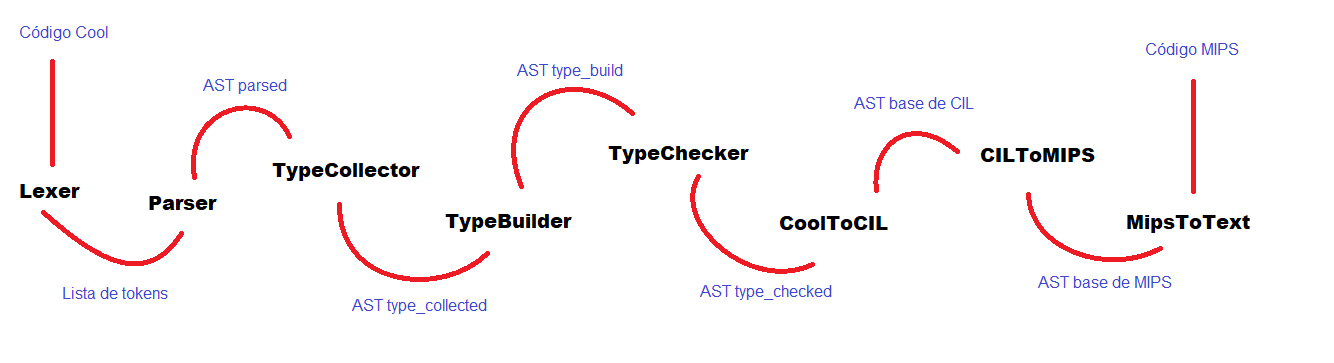
\includegraphics[width=0.9\linewidth]{./4}
\caption{}
\label{fig:4}
\end{figure}

El proceso se realiza de izuierda a derecha, recibiendo código de COOL y retornando código de MIPS. En letra negra se tiene el lexer, el parser y los visitors. En letra azul se tiene la entrada y salida de cada uno.

\section*{Lexer y Parser}
La implementación del lexer y el parser se realizó utilizando la biblioteca sly, una version mas actualizada de ply. Esta permite la definición de los tokens y la grámatica a partir de clases y decoradores que se aplican a los metodos que luego manejarán la estructura resultante. Es importante destacar que en el parser es donde se decidió resolver los nodos de tipo call que omiten la expresion sobre la que se invoca el método, añadiendo un nodo variable con referencia a self en su lugar.

\subsection*{Jerarquía de AST}
Como se mencionó anteriormente, los AST´s de la carpeta $cool$ cumplen con una jerarquía. Siendo $base$ el ancestro mayor. De esta forma, los nodos de todos los AST's serán descendientes de los nodos definidos en $base$. Luego, no fue necesario reescribir el código de los AST que sirven de entrada y salida para cada visitor (los cuales tienen, potencialmente, sutiles diferencias entre ellos). Si un la definición de un nodo de un AST no cambia con respecto al de la pasada anterior, este hereda de ese nodo anterior sin necesidad de redefinirlo. Si un nodo cambia con respecto a la pasada anterior, entonces heredará del nodo de $base$ correspondiente y se redefinirá.\\

\begin{lstlisting}
class CoolFeatureNode(type_collected.CoolFeatureNode):
    pass


class CoolAttrDeclNode(base.CoolAttrDeclNode):
    def __init__(self, lineno, columnno, attr_info, body=None):
        super().__init__(lineno, columnno)

        self.attr_info = attr_info
        self.body = body
\end{lstlisting}

Tenemos estos dos nodos del AST $type\_collected$. La definición de \code{CoolFeatureNode} es igual a la del AST de la pasada anterior ($parsed$), por tanto, se hereda de este y no se redefine su constructor. Sin embargo, \code{CoolAttrDeclNode} de $type\_collected$ necesita dos atributos que no están en el constructor de \code{CoolAttrDeclNode} de $parsed$ y por tanto, este constructor es definido mientras el nodo hereda del nodo base. Con esta estructura, se mantiene una jerarqía en la cual todos los nodos son descendientes de \code{CoolAstNode} de $base$ y sus constructores cumplen con sus entradas de línea y columna.

\subsection*{TypeCollectorVisitor}
Durante esta pasada se visitan los nodos del AST $parsed$. Visitando \code{CoolProgramNode} se definen los tipos b'asicos de COOL. Luego se visitan los \code{CoolClassNode} para definir un \code{Type} por cada una de estas y guardarlo en una lista. Todos los nodos del AST deben ser visitados para crear las instancias del nuevo AST correspondiente. Tanto en \code{TypeCollectorVisitor} como en \code{TypeBuilderVisitor} es necesario visitar todos los nodos a pesar de que sobre muchos de ellos sólo se crea la instancia del nuevo nodo, de lo contrario, un nodo instanciado pudiera tener como hijo o padre a un nodo de un AST de tipo distinto al suyo, comportamiento que provocaría muchísimos errores.

\subsection*{TypeBuilderVisitor}
En esta pasada se procede a construir los tipos recolectados, definiendo sus métodos y atributos. De esta forma se logra llevar constancia de los tipos declarados en cada atributo, de los tipos de retorno de los métodos y de los tipos da cada parámetro declarado en estos. Todos los tipos del programa están almacenados (instanciados) en la lista que \code{TypeCollectorVisitor} construyó.

\subsection*{TypeCheckerVisitor}
Una vez recolectados y construidos todos los tipos del programa (y almacenados en una lista), se pasa por todos los nodos para recolectar los posibles errores semánticos. Cada expresión del AST $type\_cheked$ tiene una propiedad \code{type}. Como el AST se visita Button Up (Cuando se visita un nodo, se procede primero a visitar a sus hijos antes de usar a los mismos para buscar cualquier error), en cada momento, todo nodo conoce el tipo de cualquiera de sus hijos (almacenado en la propiedad type) que ya fueron visitados y convertidos en instancias de $type\_cheked$ a partir de los nodos de $type\_built$. También se pasa como parámetro un scope a cada nodo visitado. Estos scope forman un árbol para cada clase, definiendo scopes hijos al visitar nodos tales como la declaración de métodos. Los errores son instanciados conociendo la línea y columna en que ocurren y almacenados en la lista \code{errors}. A continuación se describen los elementos más importantes que se tienen en cuenta para analizar los errores semánticos en los distintos nodos.\\

- Una declaración de atributo tendrá error si el tipo de su expresión hija (en caso de tenerla) no coincide con su tipo declarado. Los atributos declarados se guardan en el scope actual.\\

- En una declaración de método, se visita primero sus parámetros y se verifica que sus tipos coinciden con sus tipos declarados. Los parámetros se guardan en el scope durante la visita de los nodos parámetro. Luego se visita la expresión body del método con el scope actualizado y se verifica que su tipo sea igual al tipo de retorno declarado en el método.\\

- Un dispatch primero visitará la expresión cuyo tipo tiene al método a invocar (si esta expresión no existía en el código de cool, ya en este punto el parser la agregó como una expresión $id$ con valor "self") y luego se visitan los argumentos. Entonces se comprueba que el tipo de la expresión (o un ancestro) tenga un método con el nombre definido en el dispatch y que los tipos de los argumentos coincidan con los tipos de los parámetros de dicho método. Al visitar un static dispatch se hará casi lo mismo, con la diferencia de que no hay que buscar ancestros, se conoce el tipo exacto al que se le quiere llamar el método.\\

- Para el let in, se visitará cada declaración para verificar que los tipos de sus expresiones coincidan con sus tipos declarados y agregar las variables a un nuevo scope. Luego se visita el cuerpo con el nuevo scope creado y el tipo que este cuerpo retorne, es el que retorna el let.\\

- Para el case of, luego de visitar la expresión, se procede a visitar sus ramas (cada una de las cuales crea un scope nuevo definiendo la variable de su parte izquierda para entonces visitar a su expresión parte derecha). Entonces se busca y se retorna como tipo del nodo al ancestro común más bajo que tengan todos los tipos de las expresiones visitadas.\\

- El resto de los nodos se comporta de forma bastante intuitiva. El block visitará todas sus expresiones y su retorno tendrá al tipo de la última de estas. La asignación verificará la existencia del $id$ a asignar en el scope y que su tipo coincida con el tipo de la expresion de la parte derecha (después de visitarla). Las expresiones aritméticas visitarán ambos hijos para verificar que tengan tipo entero. Para el if then else se visitan las tres expresiones, luego se revisa que la expresión $if$ sea de tipo booleano y se retorna como tipo, al ancestro común más cercano de las expresiones $then$ y $else$. Las expresiones atómicas retornarán un nodo con su tipo correspondiente (el nodo variable se busca en el scope y da error si el $id$ no existe).

\section*{Generación de código}
\subsection*{CoolToCilVisitor}
El Los nodos del AST de CIL son los mismos dados por los profesores en tercer año, con ligerísimas modificaciones. Para armar los nods del AST de MIPS seguimos la idea de que todos los espacios de memoria están identificados por un string único. Cada vez que se visita un nodo de tipo expresión, teniendo en cuenta que el resultado de evaluar una expresión siempre termina guardado en un espacio de memoria, entonces el resultado de cada visit a expresiones será un string (el espacio de memoria que apunta al resultado). Al inicio de $cool\_to\_cil.py$ se tiene una serie de funciones auxiliares útiles para manejar el estado y registrar en lo que luego será el .data de MIPS, los objetos necesarios en los distintos casos.
Es importante destacar la visita a \code{ProgramNode} para generar las funciones builtin y algunas que necsitan un manejo especial. Estas functiones son implementadas directamente utilizando nodos del AST de CIL, donde tenemos acceso a algunos nodos especiales que tendrán un significado diferente al generar el codigo MIPS y que deben ser accesibles al programador de COOL. Como ejemplo de esto tenemos la generación de la funcion \code{type\_name}, la cual se genera para cada tipo simulando un override la funcion \code{type\_name} de Object, otro ejemplo de esto es la generación de un constructor para el tipo \code{Void}, lo cual facilita mucho el resto del trabajo con los tipos, dado que no necsitamos en muchos casos manejarlo de forma especial.

La implementacion del \code{CaseOf} resultó interesante, dado que en tiempo de ejecución resulta complejo resolver la relacion de herencia entre los tipos, y por tanto sería engorroso resolver la rama del \code{CaseOf} que se debe ejecutar; lo que hacemos es que en tiempo de compilacion generamos el equivalente a una serie de if-else para todos los posibles tipos derivados del tipo estático del objecto sobre el cual se esta haciendo pattern-matching y para cada caso resolvemos en tiempo de compilación la rama que debería ejecutarse y generamos su codigo en el cuerpo de correspondiente de la condicional.


\subsection*{CilToMipsVisitor}
Los nodos instrucciones del AST de MIPS tienen una propiedad común $comment$ sólo utilizada para el debuggeo. Los nombres de los registros se definen al inicio para facilitar el acceso a estos como se muestra a continuación.

\begin{lstlisting}
REGISTER_NAMES = ["t0", "t1", "t2", "t3", "t4", "t5", "t6", "t7", "t8", "t9"]
ARG_REGISTERS_NAMES = ["a0", "a1", "a2", "a3"]

INSTANCE_METADATA_SIZE = 4

REGISTERS = [mips.RegisterNode(name) for name in REGISTER_NAMES]
ARG_REGISTERS = [mips.RegisterNode(name) for name in ARG_REGISTERS_NAMES]
FP_REG = mips.RegisterNode("fp")
SP_REG = mips.RegisterNode("sp")
RA_REG = mips.RegisterNode("ra")
V0_REG = mips.RegisterNode("v0")
V1_REG = mips.RegisterNode("v1")
\end{lstlisting}

Al indexar REGISTERS entre 0 y 9, se obtienen los registros de propósito general y al indexar ARG$\_$Registers entre 0 y 3, se obtienen los registros que normalmente se usan para argumentos. El resto de los registros tienen nombres sugerentes, tales como V0$\_$REG. La clase MemoryManager maneja los registros que en cada momento están libres y ocpuados, con métodos para obtener registros, copiar el estado actual y retornar el estado a uno previamente copiado.\\
Al visitar el \code{ProgramNode} de CIL, se visitan primero los dotdata (\code{DataNode}) para llenar la sección .data de MIPS con los strings almacenados estáticamente y los dottypes (\code{TypeNode}) para construir en .data la tabla de métodos virtuales para los llamados a función que no sean estáticos. A continuación se muestra la tabla de métodos virtuales para el prohrama "hello world":

\begin{figure}[H]
\centering
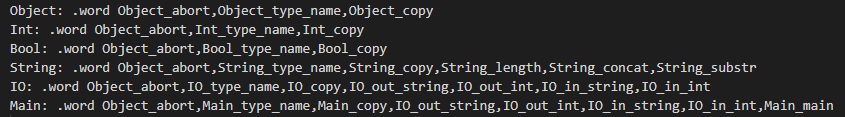
\includegraphics[width=0.9\linewidth]{./5}
\caption{}
\label{fig:5}
\end{figure}

Por cada \code{TypeNode} que se visite, se pone en .data una línea con el nombre del tipo, ".word" como tipo de almacenamiento y una serie de lables separados por coma, uno por cada método del tipo en cuestión. Al buscar en la dirección de memoria representada por un label con el nombre de cada tipo, sumada con el índice del método (se tiene la información de los índices de los métodos, dados por el orden en que fueron declarados en un tipo) multiplicado por 4, se accede a un word que en el que está la dirección de memoria del método que se quiere llamar dinámicamente. Esta tabla es necesaria pues en los llamados virtuales, es posible que hasta tiempo de ejecución no se conozca el tipo de la expresión a la que se le está haciendo dispatch y por tanto, que definición de método es la que se quiere llamar.\\
Luego de terminada la sección .data, se procede a visitar todas las instrucciones de CIL para convertirlas en instrucciones MIPS. Cada visita a un nodo instrucción retornará una lista con los nodos MIPS que equivalen a esa instrucción de CIL. A continuación se explican los aspectos más importantes de los llamados a funciones, el manejo de las direcciones de memoria y el uso de la tabla de métodos virtuales:\\

- Al visitar un FunctionNode se agrega primeramente un nodo label para marcar el inicio del método y poder saltar hacia él. Luego se agregan instrucciones para salvar en un registro el valor actual del registro FP y se mueve hacia FP el valor actual del SP (la pila). Luego se guardan en la pila las variables locales (cada una 4 bytes), se guarda el valor del registro RA para saber hacia dónde tiene que retornar el método actual en caso de que una de las instrucciones del mismo sea un llamado a otro método y se guarda el valor que se había salvado previamente del FP para no perder el FP anterior luego de retornar. En este punto, el FP marca la dirección del método en la pila, de forma que hacia abajo están los argumentos que se guardaron en esta antes de llamar a la función (4 bytes or cada uno) y hacia arriba todas las variables locales, seguidas por el RA anterior, seguido a su vez por el FP anterior\\
Siempre se lleva, mediante dos listas, rastreo de los parámetros y variables locales de la función actual en cada momento. Esas listas son salvadas al inicio del function node para restaurarlas al retornar. Al inicio de la visita se llenan estas listas iterando por los params y los locals del FunctionNode de CIL. Luego, para acceder a estos parámetros y variables locales, se usa el método \code{search\_mem} que dado el id que se quiere buscar, retorna el índice a sumarle al FP para encontrar la dirección de memoria de la variable guardada. Si es un parámetro, el índice será negatico, si es un local, será positivo y en ambos casos múltiplo de 4.\\
Una vez trabajada la pila, se procede a visitar a todas las instrucciones que están en el cuerpo de la función. La restauración de la pila a su estado anterior al llamado de la función es tarea de la instrucción \code{ReturnNode}. Se recuperan los valores previos del FP y del RA, se sacan las variables locales de la pila, se guarda en la pila la dirección al valor de retorno del méodo y se salta al RA recuperado para retornar.\\

- En el caso de los \code{StaticCallNode}, simplemente se usa una instrucción jalr para saltar al label dado y guardar en RA la dirección actual. Una vez retornado del salto, se saca de la pila el valor de retorno para almacenarlo en la dirección de memoria del local destino dado, y se saca de la pila los argumentos que fueron pusheados en esta al visitar los \code{ArgNode}. En el caso de los \code{DynamicCallNode}, se produce un comportamiento similar, con la diferencia de que no se tiene el label del método a llamar. En este caso se busca la dirección del tipo obtenido con un \code{TypeOfNode} y con el índice del método, se accede a la dirección de memoria del método en cuestión, guardada en la tabla de métodos virtuales.\\

Otro aspecto importante a explicar es la reserva dinámica de memoria para instanciar los tipos. En \code{AllocateNode} se reserv una cantidad de memoria igual a la cantidad de atributos del tipo a instanciar +1, multiplicado por 4. En los 4 primeros bytes de la dirección de la instancia se guarda la dirección del tipo (label con el nombre), y luego se le suma 4 a esta dirección de la instancia. De esta forma, al buscar en la direcc. Lo que se retorna es una dirección de memoria que tendrá en -4 la dirección del tipo instanciado y en adelante espacio reservado para los atributos de este. Al visitar \code{TypeOfNode}, basta con buscar en la dirección -4 de la instancia para conocer su tipo. Los tipos básicos de cool tienen comportamientos especiales a la hora de ser instanciados. Al no tener atributos, sólo se guarda la dirección del tipo en -4 y en 0 la dirección del valor. Por ejemplo, si es un entero, la dirección apunta a un word, si es un string, al inicio de los bytes que tienen a los caracteres de este (el string se toma hasta encontrar un 0)\\

El resto de los nodos tienen comportamientos más intuitivos para cumplir con las instrucciones de CIL respectivas. Se puede destacar los nodos \code{ConcatNode}, \code{LengthNode} y \code{SubstrinNode} por los extensos tamaños de sus códigos de visita, pero es simplemente mucha lógica de MIPS que no es importante explicar.

\subsection*{MipsToTextVisitor}
Visitor muy sencillo. Cada nodo del ast de MIPS tiene una forma de imprimirse. A estas alturas no queda proceso complicado por realizar.

\section*{Boxing y Unboxing}
Todos nuestros tipos incluyendo los tipos básicos están almacenados en el Heap y en una instancia exactamente igual a la de los tipos definidos por el usuario. El usuario por supuesto no tiene acceso para modificar los attrs en estos tipos básicos. En el momento de realizar operaciones entre estos tipos, se traen a la pila, se realiza la operacion y se crea una nueva instancia en el Heap donde se almacena el resultado.




\end{document}